%
% kurve.tex -- elliptische Kurven
%
% (c) 2021 Prof Dr Andreas Müller, OST Ostschweizer Fachhochschule
%
\bgroup
\begin{frame}[t]
\setlength{\abovedisplayskip}{5pt}
\setlength{\belowdisplayskip}{5pt}
\frametitle{Elliptische Kurven}
\vspace{-20pt}
\begin{columns}[t,onlytextwidth]
\begin{column}{0.48\textwidth}
\begin{center}
\uncover<5->{%
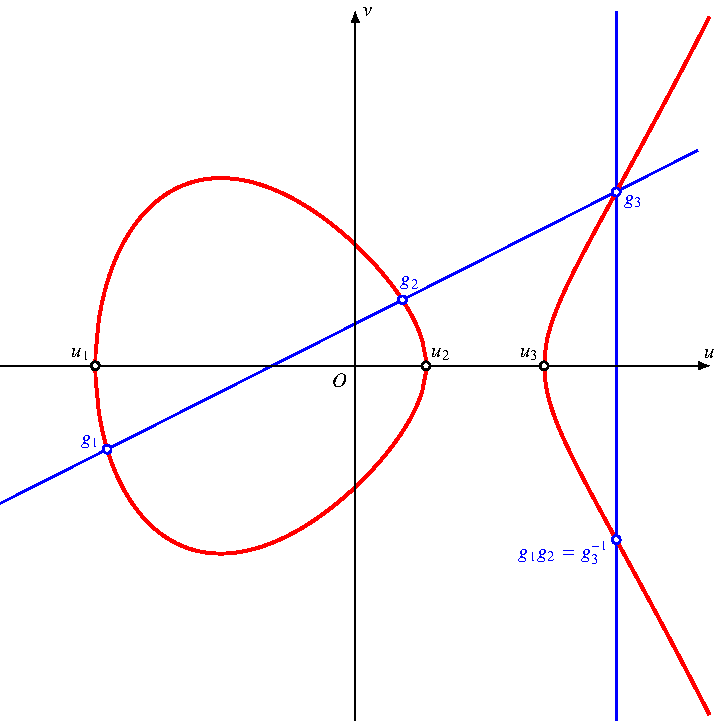
\includegraphics[width=\textwidth]{../../buch/chapters/90-crypto/images/elliptic.pdf}
}
\end{center}
\end{column}
\begin{column}{0.48\textwidth}
\begin{block}{Allgemein}
mit $a,b\in\Bbbk$
\[
Y^2 + XY = X^3 + aX + b
\]
\end{block}
\vspace{-10pt}
\uncover<2->{%
\begin{block}{Spezielle Parametrisierung}
\vspace{-10pt}
\begin{align*}
Y^2 + XY + \frac14X^2
&=
X^3 + \frac14X^2 + aX + b
\\
\uncover<3->{
(Y+\frac12X)^2
&=
X^3 + \frac14X^2 + aX + b
}\\
\uncover<4->{
v^2
&=
u^3+Au+B}
\end{align*}
\uncover<4->{mit
\[
v=Y+{\textstyle\frac12}X,
\qquad
u=X-\frac1{12}
\]}
\end{block}}
\end{column}
\end{columns}
\end{frame}
\egroup
